%\documentclass[a4paper,12pt]{article}
\documentclass{llncs}
%\documentclass[12pt]{paper}
%\documentclass[a4paper,twoside,twocolumn]{article}
\usepackage{authblk}

\usepackage[utf8x]{inputenc}
\usepackage[english]{babel}
\usepackage{subfigure}
\usepackage{float}
\usepackage{placeins}
\usepackage{graphicx}
\usepackage{array}
%\usepackage[]{algorithm2e}
\usepackage{setspace}
\usepackage{xspace}
\usepackage{cite}
\usepackage[show]{notes}
\usepackage{comment}
%\onehalfspace % interlinea 1.5
%\doublespace % interlinea 2
%\usepackage[stdsize,thm]{botex}
%\usepackage{amsthm}
%\theoremstyle{plain}
%\newtheorem{thm}{Theorem}[chapter]
%\newtheorem{cor}[thm]{Corollary}

%\newtheorem{lem}[thm]{Lemma}
%\newtheorem{prop}[thm]{Proposition}
%\theoremstyle{definition}
%\newtheorem{defn}{Definition}[chapter]
\usepackage{hyperref}
%\usepackage[bookmarksopen,bookmarksdepth=2,breaklinks=true]{hyperref}

\newcommand{\AlgFont}[1]{\textbf{#1}}

\newcommand{\GB}{\AlgFont{GB}\xspace}
\newcommand{\ADA}{\AlgFont{ADA}\xspace}
\newcommand{\BAG}{\AlgFont{BAG}\xspace}
\newcommand{\DT}{\AlgFont{DT}\xspace}
\newcommand{\RF}{\AlgFont{RF}\xspace}
\newcommand{\NAIVE}{\AlgFont{NAIVE}\xspace}
\newcommand{\MNB}{\AlgFont{MNB}\xspace}
\newcommand{\LOG}{\AlgFont{LOG}\xspace}
\newcommand{\COMB}{\AlgFont{COMB}\xspace}
\newcommand{\LDA}{\AlgFont{LDA}\xspace}
\newcommand{\LGBM}{\AlgFont{LGBM}\xspace}
\newcommand{\CAT}{\AlgFont{CAT}\xspace}

\newcommand{\MeasuresFont}[1]{\textbf{#1}}

\newcommand{\TP}{\MeasuresFont{TP}}
\newcommand{\FP}{\MeasuresFont{FP}}
\newcommand{\TN}{\MeasuresFont{TN}}
\newcommand{\FN}{\MeasuresFont{FN}}
\newcommand{\Precision}{\MeasuresFont{Pr}}
\newcommand{\Recall}{\MeasuresFont{Re}}
\newcommand{\FOne}{\MeasuresFont{F1}}
\newcommand{\AUC}{\MeasuresFont{AUC}}
\newcommand{\Kappa}{\MeasuresFont{Kappa}}
\newcommand{\MCC}{\MeasuresFont{MCC}}
\newcommand{\Accuracy}{\MeasuresFont{Acc.}}



\title {Companies default risk prediction with highly interpretable tree-ensemble machine learning model}
\author{Aris Anagnostopoulos\inst{1}\thanks{Partially supported by ERC Advanced
    Grant  788893 AMDROMA ``Algorithmic and Mechanism Design Research in Online Markets.''}  \and Stefano
  Piersanti\inst{1}\inst{2}  \and Valerio Evangelisti\inst{1}}

\institute{
Sapienza University of Rome, Italy.
  \email{aris@diag.uniroma1.it,  piersanti@diag.uniroma1.it evangelisti.1774528@studenti.uniroma1.it}
\and Bank of Italy - Statistical Data Collection and Processing Directorate
}



\begin{document}

\maketitle


\begin{abstract}



Finding a model to predict the default risk of a firm is a well-known topic over the financial and data science community. Many modern approaches triumph in finding well-performing models to forecast it. Those models often act like a black-box and don't give to financial institutions the fundamental explanations they need for their choices.
This paper aims to find a robust predictive model using a tree-based machine learning algorithm which flanked by a game-theoretic approach can provide sound explanations of the output of the model. Our study uses in combination, for the first time, two large and sparse datasets of credit data from the Italian Central Credit Register of Bank of Italy and from ECB AnaCredit survey that contain information on all Italian companies' past behaviour towards the entire Italian banking system. 
In the end, we show how our model outperforms the current predictions made by institutions and at the same time, provides insights on the reasons that lead to a particular outcome.




%In line with the results of \cite{altman-bankruptcy-17} we find that
%bagging, boosting, and random forest models outperform the others
%techniques, in particular logistic regression. In this sense also our
%research related to default prediction adds to the discussion of the
%continuing debate about superiority of computational methods over
%statistical techniques.


\end{abstract}


%\chapter{Abstract}

\section{Introduction}
\label{sec:intro}

Bankruptcy prediction of a company is, not surprisingly, a topic that
has attreacted a lot of research in the past decades by multiple
disciplines~\cite{altman-bankruptcy-17,kumar-review-07,chen-bankruptcy-11,lee-bankruptcy-13,erdogan-bankruptcy-13,cho-bankruptcy-10,wang-bankruptcy-11,Altman-8,Ohlson-9,Begley-10,Lee-10a,Fernandez-11,Odom-13,Atiya-15,Wang-16}.
Probably the main importance of such research is in bank lending.
Banks need to predict the possibility of default of a potential
counterparty before they extend a loan.
An effective predictive system can lead to a sounder and profitable
lending decisions leading to significant savings for the
banks and the companies and, most importantly, to a stable financial
banking system.
A stable and effective banking system is crucial for
financial stability and economic recovery as well highlighted by the
recent global financial crisis and European debt crisis.
%The magnitude of bankruptcy costs is a critical issue in terms of
%capital structure theories.
\notes[Aris]{It would be good if we can put a number (and a citation) on
the cost of bankrupt companies on the banking system.}

\notes[ste]{"But in Italy where families and businesses are financed mainly by credit, the wave of corporate bankruptcies and the sharp rise in unemployment have been reflected in an increase in bad debts, and consequently in a worsening of the banks' financial situation.
The growth of the new deteriorated bank loans and the slowness of the judicial recovery procedures have determined a rapid increase in the stock of these assets, which in 2015 reached a peak of 200 billion, equal to 11 percent of total loans."  (Fabio Panetta, Deputy Governor of the Bank of Italy - Rome - Camera dei Deputati - May 2018)}

Of course, despite the pletora of studies, predictiong the failure of a
company is a hard task, as demonstrated by the 
enormous increase in large corporate failures in
the last decades.

%
%
%It has also crucial importance to predict
%probability of bankruptcy in the assessment of companies’
%creditworthiness.
%
% has revealed the importance of bankruptcy prediction
%and enforced to improve new techniques.
%
%The keystone studies of
%bankruptcy literature, different findings and views regarding
%problematic issues of bankruptcy are presented in several studies.
%
%The
%inconclusive results indicate that bankruptcy prediction will remain an
%attractive field for all parties of financial world.
%Therefore, the accurate prediction of bankruptcy remains in any case a
%very important problem in financial and banking management. Basically,
%it is a binary classification problem, which includes two classes
%namely \textit{bankrupt} and \textit{non-bankrupt}. 

\notes[Aris]{Stefano, please check the paragraph below.}
\notes[ste]{OK good}

Most related research has focused on \emph{bankruptcy} prediction, which
takes place when the company officially has the status of being unable
to pay its debts (see Section~\ref{sec:problem}). However, companies
often signal much earlier their financial problems towards the banking
system by going in \emph{default}. Informally speaking, a company enters
into a default state if it has failed to meet its requirement to repay
its loans to the banks (see Section~\ref{sec:problem}). Entering into a
default state is a strong signal of a company's failure: typically banks
do not finance a company into such a state and it is correlated with
future bankruptcy.

In this paper we use historic data for predicting whether a company will
enter in default. We base our analysis on two sets of data. First, we
use historic information from \emph{all the loans} obtained by \emph{almost all
the companies} based in Italy (totaling to around $800K$ companies).
This information includes information on the companies credit dynamics in the past
years, as well as past information on relations with banks and on values of protections related to loans
\notes[Aris]{what should we write here?}
\notes[ste]{I add some concepts}
Second, we combine these data with the balance sheets of $300K$
of these companies (the rest of them are not obliged to produce balance
sheets). We apply multiple machine-learning techniques, showing that the
future default status can be predected with reasonable accuracy.
Note that the dimensions and the information in our dataset exceeds
significantly those of past work, allowing to obtain a very accurate
picture of the possibility to predict over various economic sectors.


\paragraph{Contributions.} To summarize the contributions of our paper
\begin{enumerate}
\item We analyze a vary large dataset ($800K$ companies) with granular
data (every quarter) on the performance of each company over a period of
10 year. 
\item We use these data to predict whether a company will default in the
next year.
\notes[Aris]{That's what we do, right? We go back 5 quarters, correct?
Have we tried to use data from the previous year? That is, use data from
2017 to predict what will happen in 2019.}
\notes[ste]{Yes the results are obtained using the previous 5 quarters. In particular we try to forecast default from dec 2014 to dec 2015 (for firms that are OK in dec 2014) using data from sep 2013 to dec 2014. To use more data (I've tried actually up to 5 years if I remember well) seems not improve signiificant the performance}
\item We combine our data with data available from company balance
sheets, showing that we can improve further the accuracy of predictions.
\end{enumerate}

\paragraph{Roadmap.} In Section~\ref{sec:related} we present some related
work. In Section~\ref{sec:problem} we provide definitions and we
describe the problem that we solve. In Section~\ref{sec:approach} we
describe our datasets and the techniques that we use and in
Section~\ref{sec:experiments} we present our results. We conclude in
Section~\ref{sec:conclusion}.

%
%\subsection{Bankruptcy and firms default prediction problem}
%
%Bankruptcy and firms default prediction problem are two key issues
%strongly connected.
%
%Corporate loan default prediction has become an
%increasingly important problem for financial institutions due to the
%advanced and recent financial crisis.
%
%In this article we will examine in
%particular this issue choosing a very simple approach applied to an
%Italian database containing information on credit data.
%
%To get an idea about the potential impact of the loan default prediction
%problem, we note that the volume of outstanding debt to corporations in
%the Euro area is about 5 trillion of euro.
%
%The \textit{“Non performing
%loans”} (NPL) are about 500 billions and they recently increased
%considerably as a result of the financial crisis and business
%failures.
%
%An improvement in loan default prediction accuracy of just a
%few percentage points can lead to savings of tens of billions of
%dollars.
%
%In this article we focus only on the corporate loan default prediction
%problem and we do not address prediction regarding the consumer loans
%(i.e. loan to households, for example for house purchase).
%
%Several recent and advanced techniques for predicting bankruptcy have
%been developed \cite{kumar-review-07} \cite{wang-bankruptcy-11} over the
%years.
%
%Statistical and Machine Learning techniques are the two broad
%categories used to predict bankruptcy \cite{chen-bankruptcy-11}
%\cite{kirkos-fraudulent-07}.
%
%Statistical techniques include linear discriminant analysis (LDA),
%multi-discriminant analysis (MDA) \cite{lee-bankruptcy-13}, logistic
%regression (LR), etc, while Machine learning techniques (ML) include
%well-known algorithms such as Artificial neural networks (ANN), SVM
%\cite{erdogan-bankruptcy-13}, Decision trees \cite{cho-bankruptcy-10}
%and Random Forest.
%
%\begin{figure}[H]
%
\includegraphics[width=160mm, height=60mm]{figs/CFig1.png}
%\caption{Principal techniques used to predict bankruptcy of the firms.}
%\end{figure}
%
%There are two main approaches to loan default prediction problem.
%
%The
%first approach, the structural approach, is based on modeling the
%underlying dynamics of interest rates and firm characteristics and
%deriving the default probability based on these dynamics.
%
%The second
%approach is the empirical or the statistical approach. Instead of
%modeling the relationship of default with the characteristics of a firm,
%this relationship is learned from the data.
%
%The focus of this article is on the empirical approach, especially the
%use of Decision Tree, Random Forest and others well-known Machine
%Learning techniques.
%
%Figure 1 shows the principal techniques used to address the bankruptcy
%prediction problem.
%
%
%
%
%
%
%This article is structured as follows: 
%section II contains a literature review, which briefly discusses the
%various statistical and machine   learning techniques that have been
%proposed by various researchers. Section III describes the prediction
%problem, the dataset and the techniques used for the prediction
%exercise. Section IV presents the experimental results. Finally, Section
%V concludes the paper.




\section{Related Work}
\label{sec:related}

%\subsection{A review of related work}
There has been an enormous amount of work on bankruptcy prediction. 
In order to give a flavor of how the literature that concerns bankruptcy prediction models has evolved, we briefly review the most influential previous studies below.


\subsection{Early approaches}

Initially, scholars focused on making a linear distinction among healthy
companies and the ones that will eventually default. Among the most
influencing pioneers in this field we can distinguish
Altman~\cite{Altman-8} and Ohlson \cite{Ohlson-9}, both of whom made a
traditional probabilistic econometric analysis. Altman, essentially
defined a score, the $Z$ discriminant score, which depends on several
financial ratios (working capital/total assets, retained earnings/total
assets, etc.) to asses the financial condition of a company.
Ohlson on the other side, is using a linear
regression (LR) logit model that estimates the probability of failure of
a company and identifies four main factors that affect that probability: the company’s size, its financial structure, its financial performance and its liquidity.

Some papers criticize these methods as unable to classify companies as viable or nonviable~\cite{Begley-10}. However, both
approaches are used, in the majority of the literature, as a benchmark
to evaluate more sophisticated methods.
Those sophisticated methods are the machine learning techniques which are the focus of this paper. Below, we provide a glimpse at the evolution of different techniques and at the comparison among them in the literature.

Since these early works there has been a large number of works based on machine-learning techniques \cite{lin-12, devi-18, nanni-09}.
The most successful have been based on 
decision trees \cite{Lee-10a, Zhou-10b, Gepp-10b, Martinelli-12} and neural networks
\cite{Fernandez-11, Odom-13, Boritz-14,Atiya-15,Wang-16}. Typically, all
these works use different datasets and different sets of features, depending on the dataset.

One of the first applications of the neural network methods for bankruptcy prediction, is that of Odom and Sharda \cite{Odom-13}. They compared a three perceptron network against a method that was the "rule" until then: the multivariate discriminant analysis using the Altman ratios explained above, and it proved to be more robust in terms of accuracy. Boritz et al \cite{Boritz-14} uses two different techniques to train a neural network: back-propagation and Optimal Estimation Theory (OET), and compares them to more traditional methods such as discriminant analysis, probit and logit, as well as against benchmarks provided by directly applying the bankruptcy prediction models developed by Altman and Ohlson which were previously explained. They find no superiority for neural networks; instead the performance of each technique can be improved based on the relative size of the test and train set on the nature and number of imports etc. Nevertheless, it should be mentioned that they test only one architecture of a neural network.
Atiya \cite{Atiya-15} suggests the inclusion of features extracted from equity markets because as he states “tend to be highly predictive, not only of the health of a firm, but also of the health of the economy, which in turn affects the creditworthiness of the firm”, with a resulting improvement in accuracy of around four percentage points. What we can grasp from this retrospective look of previous experiments is that, that machine learning techniques probably will perform better in our bankruptcy prediction problem, but regarding the comparison among decision trees and NNs the feelings are mixed. We cannot, though, state with certainty ex-ante which of them will be superior.

There exists a wide range of classification methods included in the category of decision trees. Lee \cite{lee-bankruptcy-13} by making a comparison of three of them using a dataset of Taiwan listed electronic companies concludes that the most efficients (in terms of accuracy) is the Generic Programming decision tree classifier which represents “a technique that applies the Darwinian theory of evolution to develop efficient computer programs (Koza ,1992)”.
Zhou and Wang \cite{Zhou-10b} on the other side, starting from the traditional random forest, propose the assignment of weights to each of the decision trees created, which are retrieved from each tree’s past performance (out-of-bag errors in training method). They show that this modification improves the performance of the algorithm in terms of overall accuracy as well as the accuracy of their balanced dataset. Gepp and Kumar \cite{Gepp-10b} turn their attention to another method, the Cox survival analysis, and compare it to the CART decision tree classifier and conclude that the former is the best one-year bankruptcy predictor, while the latter outperformed in the three-year prediction. Fernandez and Olmeda \cite{Fernandez-11} compared NN with MDA, LR, MARS and C4.5 (two well-known methods that are based on the CART decision tree algorithm) on Spanish banks and showed that NN resulted in a higher accuracy. Martinelli et al. \cite{Martinelli-12} by doing a very similar analysis on a database of Brazilian firms showed that the C4.5 algorithm is the one that outperforms the other methods.

\subsection{More recent works}

Chakraborty and Joseph (2017) train a set of models to predict distress in financial institutions based on balance sheet items, finding that ML approaches generally outperform statistical models based on logistic regression. Specifically, the RDF model allows for a marked increase in discriminatory power of about 10 percentage points in terms of the Area under the Receiver Operating Characteristic (AuROC) compared with the logit model.
Using data on US household default on mortgages, Fuster et al. (2018) find that the RDF model generates more accurate predictions than the logit model, although the improvement is minimal and accounts for about 1.2 percentage points of AuROC. The authors argue that most of these gains result from the sophisticated functional form of the RDF model, which captures the complex relationships connecting different variables to default outcomes with greater discriminatory power. 
Albanesi and Vamossy (2019) develop a model to predict consumer default based on deep learning (i.e. a combination of forecasts from deep neural network and gradient boosting) in environments with high-dimensional data (over 200 variables).
In a recent very important study, Barboza et al. \cite{altman-bankruptcy-17} compare such techniques with support vector machines and ensemble methods showing that ensemble methods and random forests perform the best.
Recently, Andini et al. ~\cite{andini-19} have used data from Italian Central Credit Register to assess the creditworthiness of companies in order to propose an improvement in the effectiveness of the assignment policies of the public guarantee programs.
The majority of the cited works typically try to predict bankruptcy of a company. Our goal is to predict both bankruptcy and bank default, after  explored the related connections between the two critical situations. Furthermore, most of these papers use balance sheet data (which are public). Our dataset contains a very granular information of a very large set of companies on the past behavior of loan repayment. In particular, we use two different important sources of credit information: the Italian Central Credit Register and, for the fist time given the novelty, the Italian component of AnaCredit, that is a very recent European credit dataset. We combine credit data with balance sheet data in order to show that the combination of the two source of information improve the prediction performances.
To our knowledge, our dataset is one of the most
extensive dataset used in the literature.
But the crucial point we wanted to address is that of trying to explain the predictions, investigating through the use of SHAP, the crucial factors that could explain the failures of companies.









\section{Methods}
\label{sec:methods}
\subsection{Feature selection}
In this part we present the technique that allowed us to find the right subset of features.\\\\
\textbf{Boruta Algorithm}

Boruta (Miron B. Kursa, Witold R. Rudnicki, 2010) is a modern feature selection algorithm which aims at lowering the probability of overfitting while at the same time promotes the most important features which will have an impact on the interpretability of the developed model. The algorithm is designed as a wrapper around a Random Forest classification algorithm. It iteratively removes the features which are
proved by a statistical test to be less relevant than random probes.\\
The Boruta algorithm consist of these following steps:
\begin{enumerate}
    \item Augment the dataset by adding shadow variables that are just copies of all variables.
    \item Shuffle the new attributes to remove their correlations with the target value.
    \item Train a random forest classifier on the extended dataset and gather the Z scores computed
    \item Find the maximum Z score $Z^*$ among the shadow attributes and then assign a hit to every attribute that scored better than that.
    \item For each variable with unknown importance perform a two-sided test of equality with $Z^*$.
    \item Set the variables which have importance significantly lower than $Z^*$ as ‘unimportant’ and permanently remove them from the dataset.
    \item Set the variables which have importance significantly higher than $Z^*$ as ‘important’.
    \item Remove all shadow attributes.
    \item Repeat the procedure until the importance is assigned for all the attributes, or the algorithm has reached the previously set limit of the random forest runs.
\end{enumerate}
\subsection{Classifiers}
\label{subsec:algorithms}

As we explain in Section~\ref{sec:related}, the first approaches for
assessing the likelihood of companies to fail were based on some fixed
scores; see the work by Altman~\cite{Altman-8}. Current approaches are
based on more advanced machine-learning techniques. In this paper we consider a set
of diverse tree-based machine-learning approaches to predict credit defaults.

In the first test we used five well-known machine-learning approaches.
We provide a brief description of each of them, as provided by
Wikipedia.

\textbf{Decision Tree (\DT)}: one of the most popular tool in decision
analysis and also in Machine Learning. A decision tree is a
flowchart-like structure in which each internal node represents a
``test'' on an attribute, each branch represents the outcome of the test, and
each leaf node represents a class label (decision taken after computing
all attributes). The paths from root to leaf represent
classification rules.

\textbf{Random Forest (\RF)}: Random forest are an ensemble learning
method for classification, regression and other tasks, that operate by
constructing a multitude of decision trees at training time and
outputting the class that is the mode of the classes. Random decision
forests correct for decision trees' habit of overfitting to their
training set.

\textbf{CatBoost(\CAT)}: Categorical Boosting (L.Prokhorenkova, Gleb Gusev et al. 2019)\cite{catboost} is a new gradient boosting algorithm that improves other standard boosting implementations. It introduce the ordered boosting algorithm, an alternative to gradient boosting based on permutation and an innovative algorithm for processing categorical features. Both of them are created to overcome a problem of target leakage present in currently implementation of gradient boosting algorithm.
\subsection{Explainability}
As we already said, understanding the reasons why a model makes a certain prediction is very important especially in financial applications. A method to be considered a good feature attribution method must be consistent and accurate.
For tree-ensamble methods like gradient boosting machine and random forest, for each input feature is possible to determine an importance value. These values are shown to be inconsistent and thus don't provide clear and definite explanation over the model's prediction.
Here we explain how a recent approach called treeExplainer is currently the best for this purpose.

\textbf{TreeSHAP}
TreeSHAP from Explainable AI for Trees by Lundberg et al. (2020) \cite{treeshap} is a modern method to provide interpretability of tree-based models. It provides the first polynomial algorithm to compute optimal explanations based on game theory that directly measure local feature interaction effects and allows to understand global model structure based on those local effects. TreeExplainer is based on Shapley values that in Lundberg and Lee (2017)\cite{shap} is proved to be the only possible method in the broad class of additive feature attribution methods to satisfy the properties of \emph{local accuracy}, \emph{consistency},  \emph{missingness}:
\begin{enumerate}
    \item Local accuracy: when approximating a model $f$ for a specific input $x$, the explanation’s attribution values $\phi_i(f,x)$ should sum up to the output $f(x)$
    \begin{equation}
        f(x) = \phi_0(f) + \sum_{M}^{i=1}\phi_i(f,x)
    \end{equation}
    \item Consistency:in presence of changes in the model, if the contribution of a feature increase or stays equal, its input's attribution should not decrease.
    \item Missingness: features with no effect on the function $f(x)$ must have no assigned impact.
\end{enumerate}
Shapley values are computed by introducing each feature, one at a time, into a conditional expectation function of the model’s output. The change produced is attributed at each step to the feature that was introduced. Then the algorithm average over all possible feature
orderings.

SHAP(SHapley Additive exPlanation) has been proved to be consistent with human intuition and are very useful due to their ability to provide insights on how each feature plays a role in a single prediction.




\section{Experimental Setup }
\label{sec:approach}

In this section we describe the data on which we based our analysis and
the evaluation measures that we used to evaluate the performance.
\subsection{Dataset Description}
\label{subsec:dataset-description}

Our analysis is based on three datasets. The first and most important in
our work is composed of information on loans and the credit of a large
sample of Italian companies. The second reports balance sheet data of a
large sub-sample of medium-large Italian companies.


\paragraph{Central Credit Register dataset.} 

The first dataset consists of a very large and high granular dataset of credit
information about Italian companies belonging to the Italian Central Credit Register (CCR).  It is an information system on the debt
of the customers of the banks and financial companies supervised by the Bank of Italy. Bank of Italy collects information on customers'
borrowings from the intermediaries and notifies them of the risk position of each customer vis-à-vis the banking system.
By means of the CCR the Bank of Italy provides
intermediaries with a service intended to improve the quality of the lending of the credit system and ultimately to enhance its stability.
The intermediaries report to the Bank of Italy on a monthly basis the total amount of credit due from their customers: data information about
loans of $30,000$ euro or more and non-performing loans of any amount.
The Italian CCR has three main goals: (1)
to improve the process of assessing customer creditworthiness, (2) to raise the quality of credit granted by intermediaries, and to (3) strengthen
the financial stability of the credit system. 

The crucial feature of this database is the high granularity of credit information.
It contains information for about $800K$ companies for each quarter. In this paper we use credit data referred to the last two years (2018--2020).
Central Credit Register data are not public.
The main features are shown in.
Table~\ref{tbl:attributes}.
%
%To the best of our knowledge, Machine Learning techniques
%have not yet been applied for the analysis of these database.
%We used a overall credit dataset containing over 800,000 rows. Each row contain credit
%data related to a single firm. For each firm the dataset contains about
%20 different attributes; the most important are shown in the following
%Table. We considered information on the dynamics
%of credit to firm with quarterly frequency. The objective of the work is
%to predict whether a company that at the time T was not in default
%status in the following year will be classified in default. The complete
%dataset used to make the predictions consists of credit information over
%a period of five years from 2009 to 2014.
%


%\begin{figure}[H]
%\flushleft
%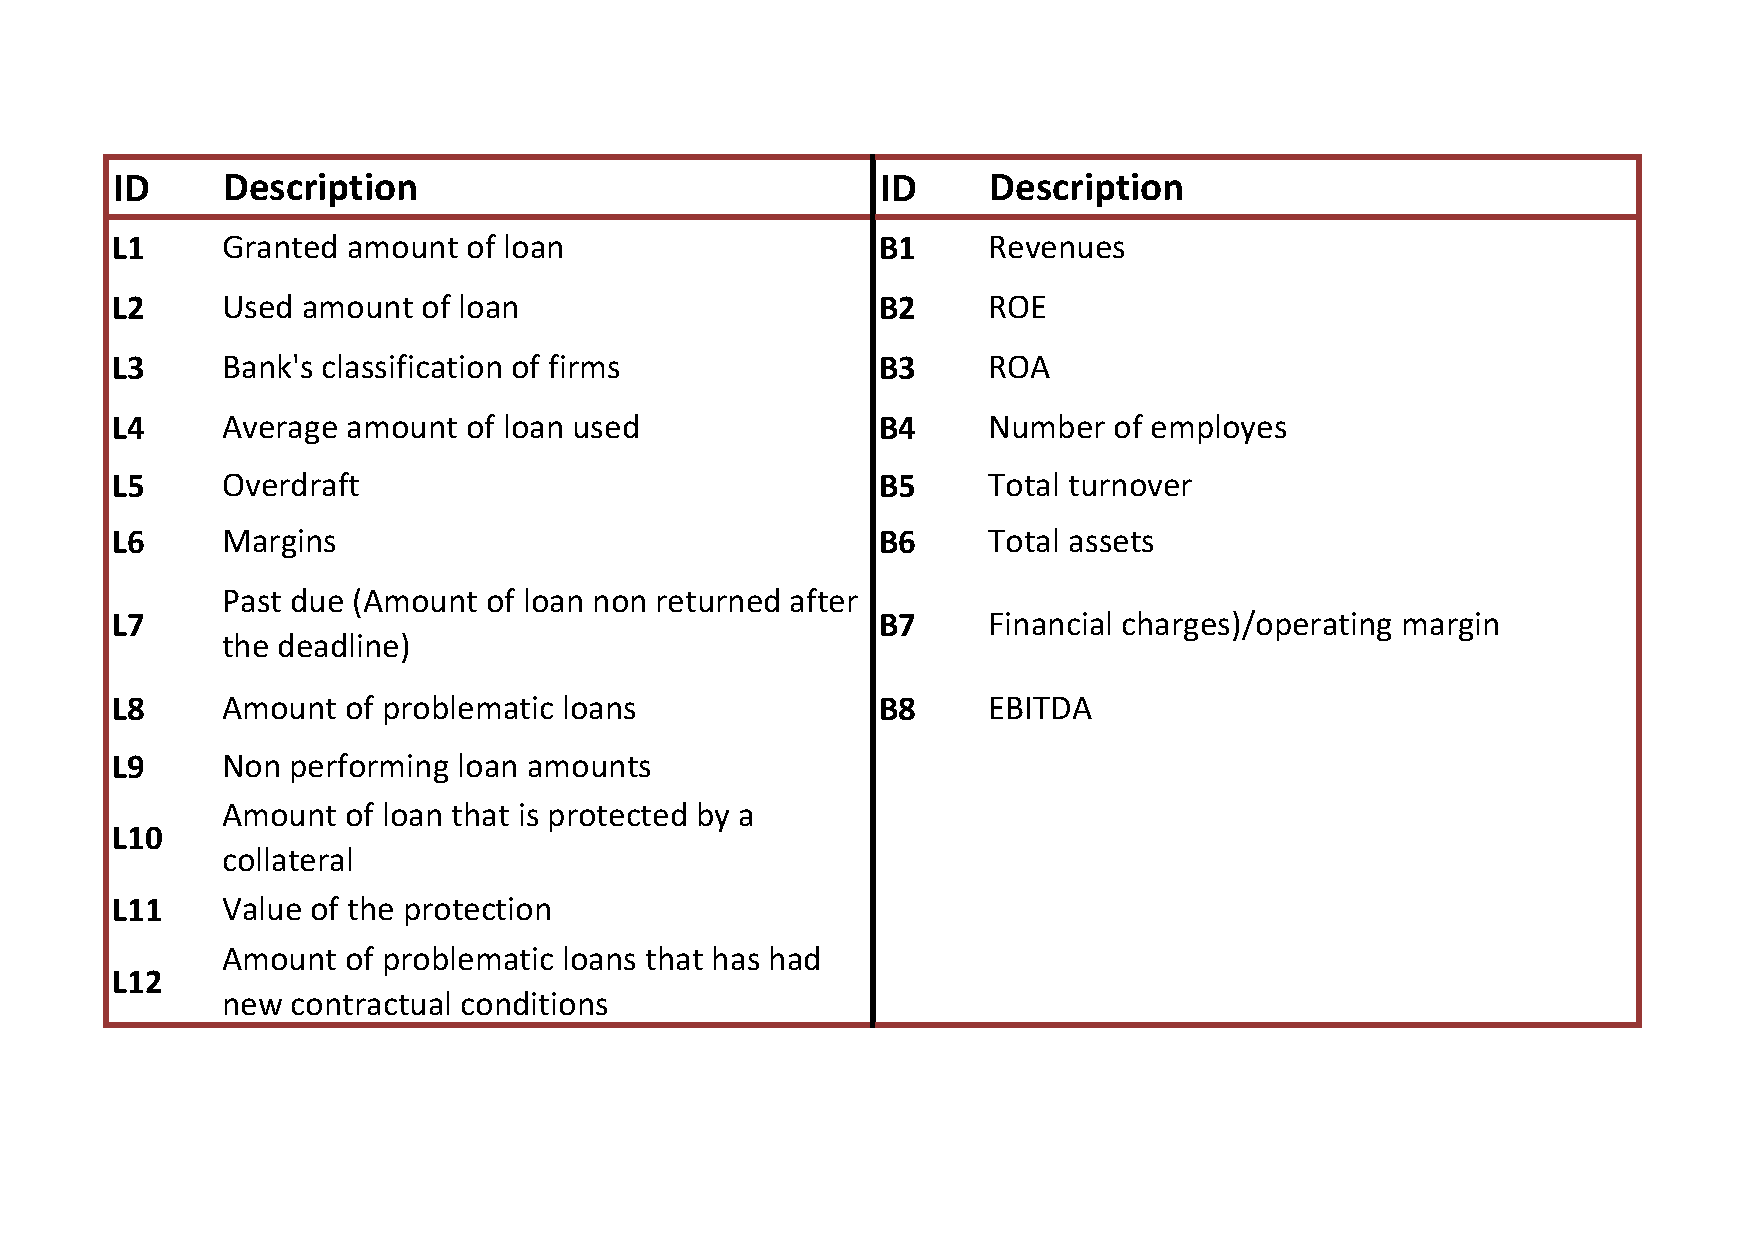
\includegraphics[width=180mm, height=80mm]{figs/Table_dataset.pdf}
%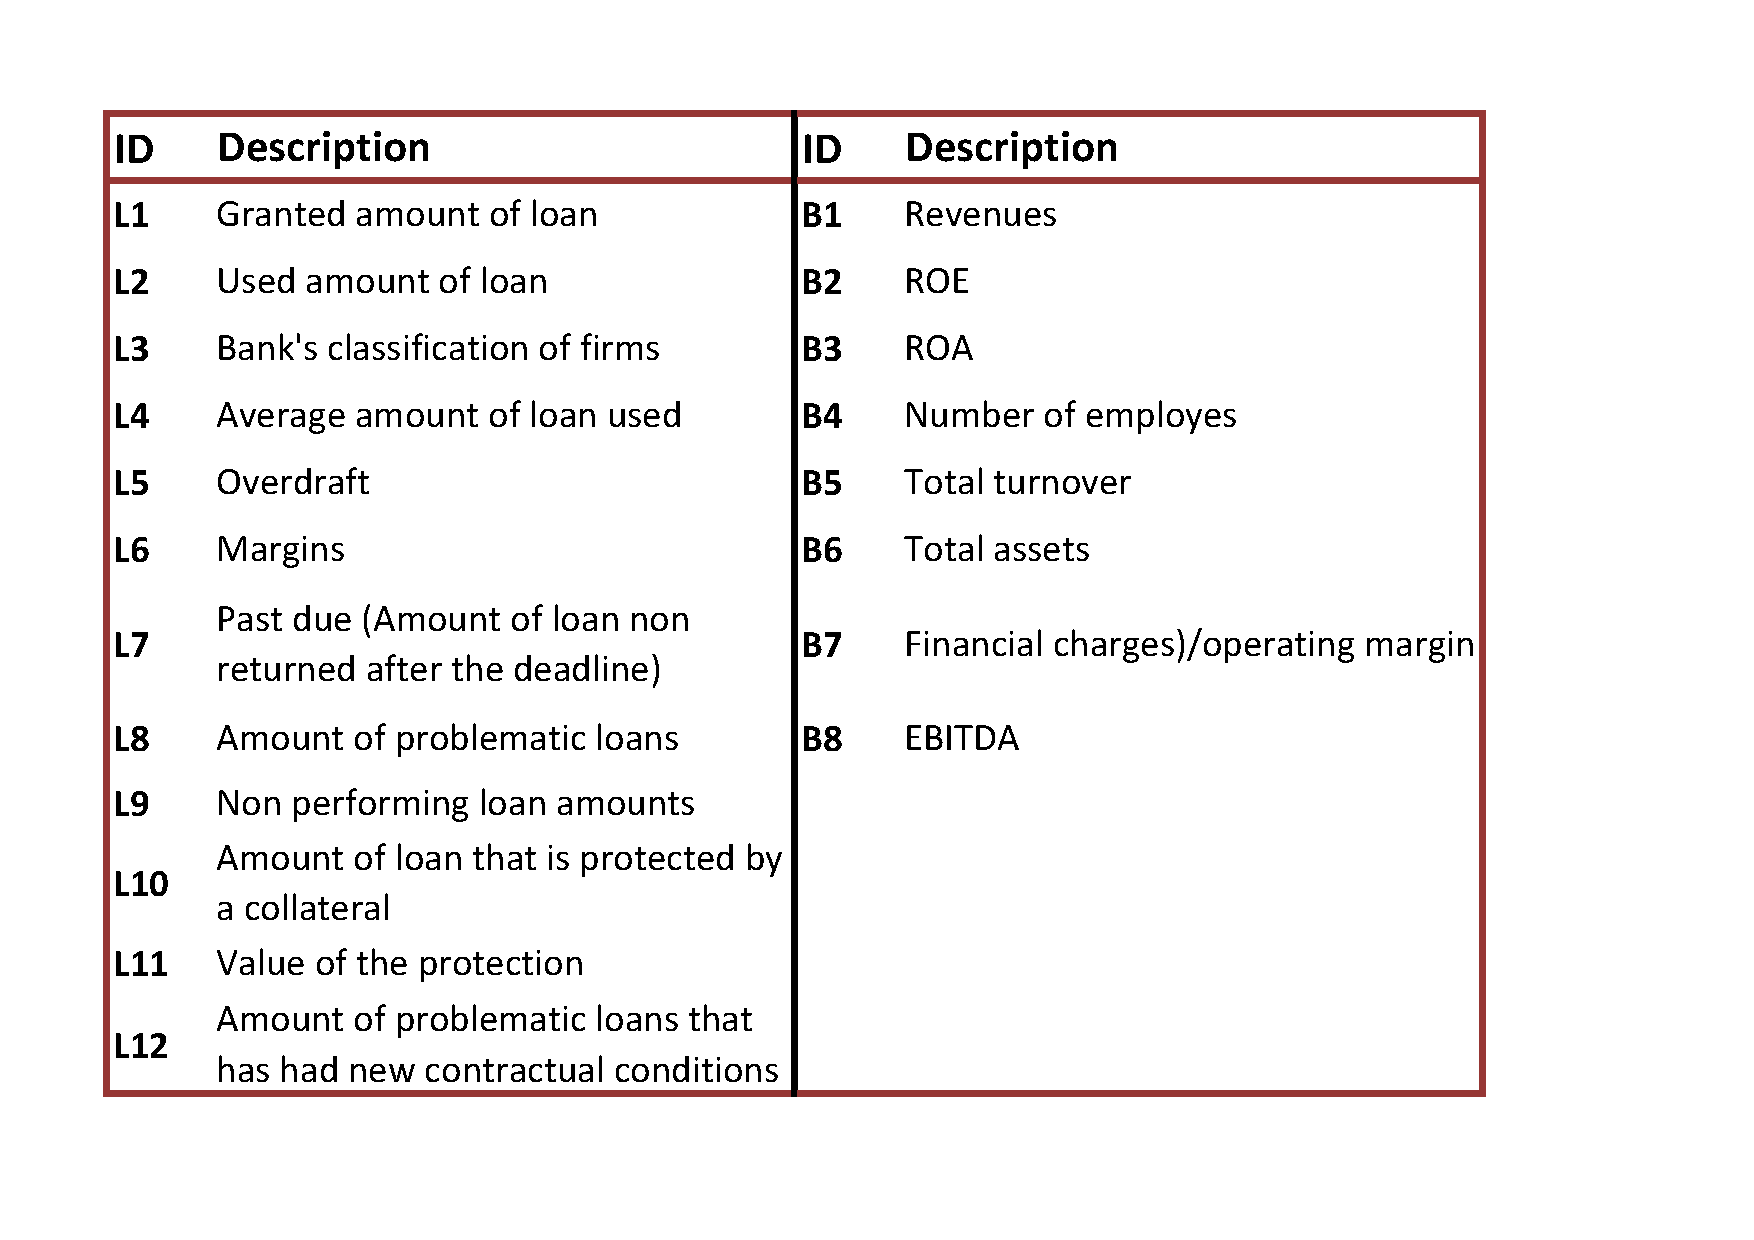
\includegraphics[width=180mm, height=80mm]{figs/Cdataset.pdf}
%\caption{Loan dataset (L) and Balance sheet dataset (B): main
%attributes. Loans data are quarterly from 2009 to 2014;
%Balance sheet data have annual frequency from 2006 to 2014}
%\end{figure}

\begin{table}
\small
\begin{center}
\begin{tabular}{ lllc | lllc }
\hline
& & & & & & &  \\
   &  \textbf{ID}       &\textbf{Description} &  & & \textbf{ID}       &\textbf{Description}   &\\
\hline
\hline
\\
&\textbf{C1}    &Granted amount of loans & & &\textbf{A1}  &Firm's default status (assessed by banks)   &  \\
&\textbf{C2}    &Used amount of loans & & &\textbf{A2}  &Loan expenses   &  \\
&\textbf{C3}    &Bank's classification of firm & & &\textbf{A3}  &Loan arrears   &  \\
&\textbf{C4}    &Average amount of loan used& & &\textbf{A4}  &Initial loan Commitment     & \\
&\textbf{C5}    &Overdraft & & &\textbf{A5}  &Outstanding nominal amount of loan    & \\
&\textbf{C6}    &Margins & & &\textbf{A6}  &Off-balance sheet amount     & \\
&\textbf{C7}    &Past due (loans not returned after the deadline) & & &\textbf{A7}  &Amount of protection   & \\
&\textbf{C8}    &Amount of problematic loans & & &\textbf{A8}  &Probability of default of firm (assessed by banks)  & \\
&\textbf{C9}    &Amount of non-performing loans & & &  &  & \\
&\textbf{C10}    &Amount of loans protected by a collateral & & &  &  & \\
&\textbf{C11}    &Value of the protection & & &  &  & \\
&\textbf{C12}    &Previous "Adjusted default" classification & & &  &  & \\
\hline
\\
\end{tabular}
\caption{Main attributes for the two credit datasets: Central Credit Register (C) and  AnaCredit (A)}
%The loan dataset contains credit data for about 800,000
%Italian firms and has quarterly frequency from 2009 to 2014. Balance
%sheet dataset contains data for about 300,000 Italian firms with
%annual frequency from 2006 to 2014. Companies for which balance
%sheet data are available represent a subset of the previous loan
%dataset consisting of the largest firms.
\label{tbl:attributes}
\end{center}
\end{table}


\begin{table}
\small
\begin{center}
\begin{tabular}{| lll | }
\hline

   &  \textbf{ID}       &\textbf{Description} \\
\hline
\hline
 &  \ & \\
&\textbf{X1}    &Revenues   \\
&\textbf{X2}    &Employees   \\
&\textbf{X3}    &Total added value  \\
&\textbf{X4}    &MOL \\
&\textbf{X5}    &Active  \\
&\textbf{X6}    &Working Capital  \\
&\textbf{X7}    &Net Equity \\
&\textbf{X8}    &ROE  \\
&\textbf{X9}    &ROI \\
&\textbf{X10}    &ROA   \\
&\textbf{X11}    & Margin on revenues \\
&\textbf{X12}    &Operating costs/production value  \\
&\textbf{X13}    &MOL/production value\\
&\textbf{X14}    &MOL/operational added value\\
&\textbf{X16}    &Liquidity\\
&\textbf{X17}    &Total equity/financial debt\\
&\textbf{X18}    &Bank financial debt+ICS/financial debt\\
&\textbf{X19}    &Financial expenses/MOL\\
&\textbf{X20}    &Ebitda/Net financial charges\\
&\textbf{X24}    &Current profit\\
&\textbf{X34}    &Net revenues/operating assets\\

\hline

\end{tabular}
\caption{Main attributes for the balance sheet dataset (X)
.}
\label{tbl:attributes}
\end{center}
\end{table}




\paragraph{The Balance-sheets dataset.}

Our second dataset consists of the balance-sheet data of about $300K$
Italian firms. They are generally medium and large companies and they
form a subset of the $800K$ companies with loan data. 
It contains balance-sheet information for years from 20013 and 2014.
The main features include those that regard the profitability of a company, such as return
of equity (ROE) and return of assets (ROA); see Table~\ref{tbl:attributes} for a more
extended list. Typically balance sheet data are public data and have been used extensively for
bankruptcy prediction (e.g., see Barboza et
al.~\cite{altman-bankruptcy-17} and references therein).

\paragraph{The AnaCredit dataset.}

The third dataset is a dataset with detailed information on individual bank loans in the euro area. The name of the dataset is “AnaCredit” and it stands for “analytical credit datasets”.
AnaCredit is a shared multipurpose database containing loan-by-loan information on credit extended by credit institutions to companies and other legal entities. On 18 May 2016 the Governing Council of the ECB adopted Regulation ECB/2016/13 on the collection of granular credit and credit risk data (AnaCredit) establishing Stage 1 of a shared database for the European System of Central Banks (ESCB) as of September 2018. The database will contain a large number of credit information, updated mostly on a monthly basis, based on harmonised concepts and definitions common to all participating countries.
AnaCredit is a shared multipurpose database that will contain loan-by-loan information on credit to companies and other legal entities extended by credit institutions and their foreign branches on a monthly basis. Based on compelling requests from   users in a large number of central banks’ business areas, AnaCredit data collection has been designed with a view to obtaining a complete picture of a) the total credit exposure of the European banks and b) the total indebtedness of borrowers across all lenders. The information collected consists of 88 different attributes based on harmonised concepts and definitions and covers various aspects of the credit exposure.

In the Table ~\ref{tbl:attributes} we can see the main features we will consider in the paper in order to try to predict firms bank default. 
This information also includes some important vulnerability indicators assessed by banks, such as default status and probability of default of companies that have relationships with banks.

\paragraph{Merged credit dataset.}

The AnaCredit dataset contains monthly information for approximately 800,000 Italian companies as of June 2018.
In order to predict bank failure we will use a combined dataset comprising data from the CCR and AnaCredit datasets. We will use data from the past two years (June 2018 to June 2020) to try to predict companies that were in a "good situation" with respect to the Italian banking system in June 2019 and that will result in Adjusted bank default in June 2020. The overall dataset we will use contains over 570,000 companies for a total of 136 features.






\begin{comment}
    

Our second dataset consists of the balance-sheet data of about $300K$
Italian firms. They are generally medium and large companies and they
form a subset of the $800K$ companies with loan data. 
It contains balance-sheet information for each year from 2006 to 2014.
The main features include those that regard the profitability of a company, such as return
of equity (ROE) and return of assets (ROA); see Table~\ref{tbl:attributes} for a more
extended list. Typically balance sheet data are public data and have been used extensively for
bankruptcy prediction (e.g., see Barboza et
al.~\cite{altman-bankruptcy-17} and references therein).
%
%Among the
%fundamental ones are those regarding the profitability of companies, as
%in the case of ROE and ROA.
%
%
%With the aim of improving the forecasts of the default status of Italian
%firms, we have also performed some classification attempts  by
%integrating credit information with some balance sheet indicator for Italian
%companies. In particular, we used a set of firms balance sheet
%indicators from the CEBI dataset: some important indicators are used
%that are very similar to those used by Barboza et al.
%\cite{altman-bankruptcy-17} also  in his famous Z-score. Among the
%fundamental ones are those regarding the profitability of companies, as
%in the case of ROE and ROA. The balance sheet dataset contains data
%related to about 300,000 Italian firms; these are generally medium and
%large companies. For each firms we used a set of eight indicators shown
%in the Table. Balance sheet data are public data.\\
%
%The three hundred thousand companies for which balance sheet data are
%available constitute a sub-sample of those belonging to the loan
%dataset. Therefore the dataset that uses both information on loans and
%balance sheet info is made up of about 300,000 companies.

\end{comment}

\paragraph{Heavy imbalanced dataset}

A lot of modern problems in the machine learning field have to deal with imbalanced datasets. For some of them, the problem is due to the lack of data samples, for others to the intrinsic nature of the problem.
While for the first group it’s easier to find a way around the problem for the second it represents a characteristic of the dataset itself and would make the prediction capability of any model much lower. 
In this case, the problem falls into the second category since we are trying to assess the likelihood of companies to fail and just a small amount of the total fail over the year. For our dataset described above, the ratio between failed and healthy companies is close to 2%.

\subsection{Evaluation criteria}
We use a variety of evaluation measures to assess the effectiveness of
our classifiers, which we briefly define. As usually, in a binary
classification context, we use the standard concepts of true positive
(TP), false positive (FP), true negative (TN), false negative (FN):
\medskip

\begin{center}
\begin{tabular}{|l|c|c|}
\hline
	& Predicted Default	& Predicted Not Default \\\hline
Default 	&\TP	&\FN	\\\hline
Did not default &\FP	&\TN	\\\hline
\end{tabular}
\end{center}
\medskip

For instance, FN is the number of firms that defaulted during a particular year but
the classifier predicted that they will not default.


We now define the measures that we use:
\begin{itemize}
\item Precision: $\displaystyle \Precision=\frac{\TP}{\TP+\FP}$
\item Recall: $\displaystyle \Recall=\frac{\TP}{\TP+\FN}$
\item F1-score: $\displaystyle \FOne=2\cdot\frac{\Precision\cdot\Recall}{\Precision+\Recall}$
%\item Type-I Error: $\displaystyle \TypeOne=\frac{\FN}{\TP+\FN}$
%\item Type-II Error: $\displaystyle \TypeTwo=\frac{\FP}{\TN+\FP}$
%\item Balanced Accuracy: $\Bacc \FOne=2\cdot\frac{\TP\cdot\TN}{\TP+\TN}$
% \item Mattews correlation coefficient: \textbf{MCC}
% \item  \textbf{Kappa}
\item Area under the ROC curve: \textbf{AuROC}
\item True positive rate: \textbf{TPR}
\item True negative rate: \textbf{TNR}
\end{itemize}

Our analysis of the results will be particularly focused on considering the AuROC, which is a particularly useful indicator for performance comparisons as it is widely used in literature.



\section{Experimental Results}
\label{sec:experiments}

\subsection{Bankruptcy prediction}

In this section, we address the problem of predicting the failures of Italian companies. Therefore our interest will be concentrated in predicting which companies will no longer be active in the following year.
Usually in the most important literature on this subject (see for example ~\cite{altman-bankruptcy-17}),  those predictions are performed using primarily balance sheet data. In this work we decided to use the combination of the balance-sheets dataset with the Central Credit Risk. Below in the comments on the results we will focus our attention on the Auroc, which is the performance indicator that we have tried to maximize in setting the algorithms.
The results obtained are shown in the table below: the Auroc, in reaches about 0.9 for the best classifiers and varies slightly depending on the classifier used (0.92 for boosting classifiers while using DT Auroc is 0.77). ML algorithms generally performs better than statistical classifiers like Logistic regression. This result confirms a well known evidence in the recent literature also for our particular dataset.

The overall dataset that we used includes at the beginning approximately 340,000 companies for a total of over 155 columns. Thanks to the use of the Boruta Algorithm for feature selection we succeeded in reducing it to a total of just 12 significant attributes.


\begin{table}[H]
\begin{center}
\begin{tabular}{lcccccccccccl}
\hline
 &AuROC & Recall & Precision  &F1-score & TPR &  TNR\\
\hline
\hline
\LOG         &0.77 &0.58 &0.005       &0.010 &0.38 &0.88 \\
 \hline
\DT         &0.77 &0.75 &0.006       &0.010 &0.78 &0.77 \\
\RF         &0.93 &0.86 &0.008      &0.016 &0.84 &0.83  \\
\CAT        &0.93 &0.88 &0.008       &0.016 &0.85 &0.83 \\
\hline
\\
\end{tabular}
\caption{Balanced training set; balance-sheet data + loan data.}
\label{tbl:bankr_unb_bal}
\end{center}
\end{table}


\subsection{Adjusted default prediction}


In this section we try to predict bank default or more precisely "adjusted default", according to the previous definition (see chapter 3.1).  
\newline
In other words, in this case we will be interested in the prediction of bank default, or in a state of serious difficulty for a company with respect to the banking system, which generally involves the company's inability to repay its bank debts. This condition of a company does not necessarily correspond to a bankruptcy but it is very important to foresee for the stability of the banking and financial system.
\newline
The experimental results are reported in the tables below.
In this case, the usual data used to make prediction are credit data. In our study we used the same merged dataset (credit + balance) as for the bankruptcy problem. 

Also in this case, due to the strong imbalance of the dataset we decided to train all the models on an under sampled dataset. The main performance indicator we have focused our analysis it is the Auroc, but we also looked at other classic indicators including the F1-score.
 We can observe how the Machine learning classifiers have better performance than the other statistical classifiers (for example Logistic Regression). In particular, considering Auroc we can obtain a gain greater than $0.15$. As mentioned before, this result is in line with other evidence in the literature (see in particular Barboza and alt.).


\begin{table}[H]
\small
\begin{center}
\begin{tabular}{lcccccccccl}
\hline
 &AuROC & Recall & Precision  &F1-score & TPR &  TNR\\
\hline
\hline
\LOG          &0.72 &0.66 &0.09       &0.15 &0.67 &0.67 \\\hline
\DT          &0.75 &0.75&0.12       &0.21 &0.74 &0.75 \\
\RF          &0.90 &0.82&0.19      &0.31 &0.83 &0.84  \\
\CAT        &0.91 &0.82&0.20       &0.32 &0.83 &0.84 \\
\hline
\\
\end{tabular}
\caption{Balanced training set;loan+balance data.}
\label{tbl:unb_loan}
\end{center}
\end{table}


Moreover, among the ML classifiers, those that obtain the best results are those of the boosting type with Catboost being the best.
We also found that trying to predict bank default using the combination of the datasets provide improved level of performance .
\newline
Based on this experimental evidence, in this case the conjecture we make is that credit data are critical to predict a bank default while balance sheet data has less predictive power in this case. However, the combination of the two sources of information can improve adjusted default prediction.


\subsection{Adjusted default prediction with AnaCredit data}

In this section, we show the first evidence using a new credit dataset from AnaCredit survey. The main results underline that the new data have good forecasting capabilities, similar to the CR loans data used in the previous predictions. We can obtain using AnaCredit data in combination with Central Credit Register data Auroc equals to $0,93$ for the best classifier.



\begin{table}[H]
\begin{center}
\begin{tabular}{lcccccccccccl}
\hline
 &AuROC & Recall & Precision  &F1-score & TPR &  TNR\\
\hline
\hline
\LOG         &0.86 &0.87 &0.05       &0.10 &0.80 &0.66 \\
 \hline
\DT         &0.78 &0.78 &0.07       &0.12 &0.79 &0.78 \\
\RF         &0.92 &0.83 &0.11      &0.19 &0.84 &0.86  \\
\CAT        &0.93 &0.84 &0.11       &0.19 &0.84 &0.86 \\

\hline
\\
\end{tabular}
\caption{Balanced training set; Anacredit + Central Credit Register.}
\label{tbl:unb_anac}
\end{center}
\end{table}




The complete dataset consists of $573,000$ rows and $136$ columns that after feature selection is reduced to $16$ .
Since the AnaCredit dataset is very recent (starting from September 2018) in this exercise we will use data relating to the last few years (from 2019 to 2020). It will therefore not be possible to use balance sheet data as these are not yet available.



\subsection{Evaluation of results: default prediction based on banks Probability of Default}

In order to evaluate the performance of Machine learning classifiers, we would compare the previous predictions with a prediction performed using the "Probability of default" that is reported from the Italian banks in AnaCredit. In particular we assume that we will predict a default if a firm has a probability of default greater than an established threshold.
The prediction results show a very low performance demonstrating the difficulty of the default prediction problem. The best prediction results we obtain are in correspondence with the PD threshold equal to 0.1 (i.e. assuming as default the companies that the previous year have a PD greater than 0.1) but also in this case it is not possible to obtain an Auroc greater than 0.7.


\begin{figure}[H]

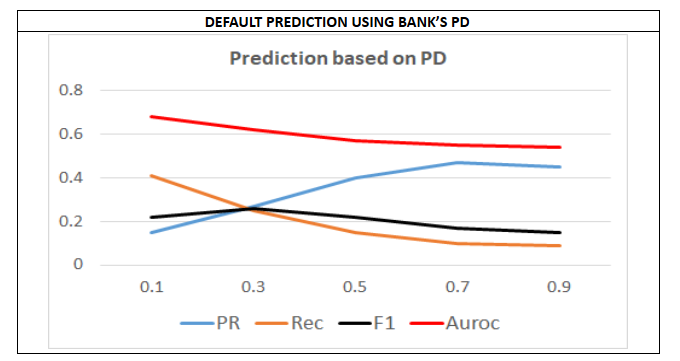
\includegraphics[width=120mm, height=80mm]{figs/PD.png}

\caption{Adjusted default prediction based on bank's PD}
\end{figure}

As we have seen above, the Probability of Default is one of the most relevant forecasting factors even using ML algorithms. But the use of these techniques, in particular the tree-ensemble algorithms, provide a significant performance gain with an Auroc higher than 0.93.


\subsection{Explainability}
In this section we use SHAP in order to show an analysis of the predictions regarding both Bankruptcy and Adjusted default.

\paragraph{Bankruptcy}

We analyze Bankruptcy predictions that we obtained using the combination of balance sheet data and credit data. In this case we consider our best performing model CatBoost.
From the explanatory overview we can observe the most important features that determine the forecast: the "rating" appears to be the most relevant one together with other features (X20-"EBITDA/Net financial charges" and X14-"MOL/operational added value") from the balance sheet dataset, but also the overdrafts ("scoperto") also plays an important role.

Usually bankruptcy predictions are made using only balance sheet attributes, from our overview we can definitely say that credit data can really be meaningful with a clear explanatory power even though balance are still the most of the important attributes.

\begin{figure}[H]
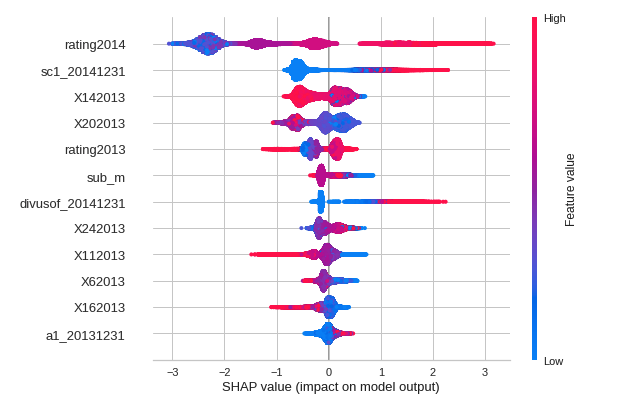
\includegraphics[scale = 0.7]{latex/figs/bankrupt_exp.png}
\caption{Explanatory overview Catboost}
\end{figure}

SHAP values allows us to see also in detail the effect of each attribute on a single prediction.
In the example below we can see how the prediction of an healthy organization is primarily driven by a very low rating bot in 2014 and 2013 and an overdraft equal to zero.
\begin{figure}[H]
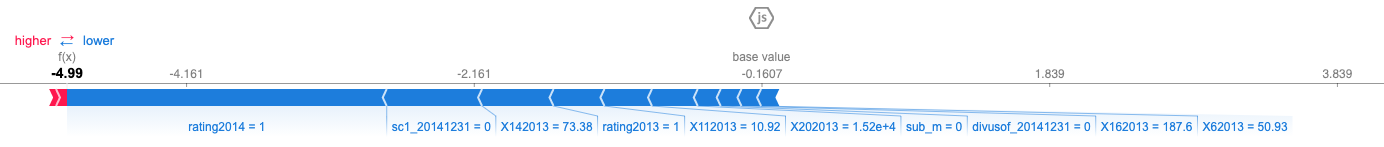
\includegraphics[scale=0.4]{latex/figs/bankrupt1_exp.png}
\caption{Explanation of a single negative prediction}
\end{figure}
In this other example instead is possible to see that the prediction of this firm as failed is due to the high rating in 2014 and 2013 while at the same time to the high overdraft and the decrease over the year of its margins.
\begin{figure}[H]

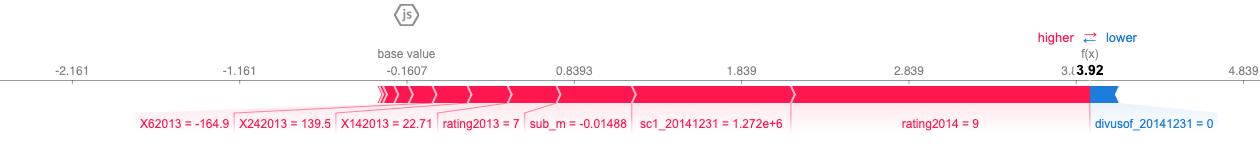
\includegraphics[scale=0.4]{latex/figs/bankrupt2_exp.png}
\caption{Explanation of a single positive prediction}
\end{figure}


\paragraph{Adjusted default}

Considering Adjusted default prediction, we first consider the prediction exercise we conducted using both the balance sheet and credit datasets. An analysis of the results obtained using the CatBoost classifier are shown in the following figures. Also in this case if we use other classifiers we obtain similar results. 
We can see that the most important features in prediction are again "rating" (that shows an important predictive power also for bank default) but some credit features appear decisive such as the overdraft "scoperto" (sc) and "previous default status" (pos).  
This analysis corroborates our conjecture that to predict credit default, credit data are fundamental but at the same time some balance sheet features can also improve bank default forecasts and provides a clear intepretability.


\begin{figure}[H]

%\flushleft
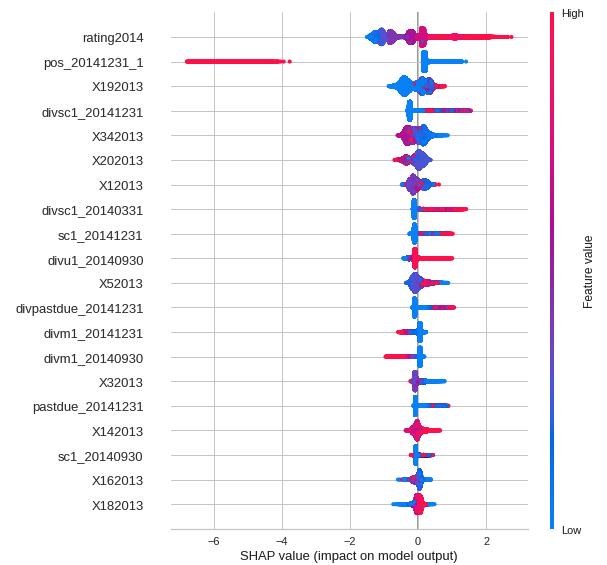
\includegraphics[scale = 0.7]{latex/figs/adjusted_exp.png}
\caption{Explanatory overview Catboost}
\end{figure}

As for the bankruptcy prediction we show how the SHAP values for both healthy and failed companies provide a clear picture of the reasons why that prediction has been made, accordingly to the explanatory overview.
\begin{figure}[H]
\flushleft
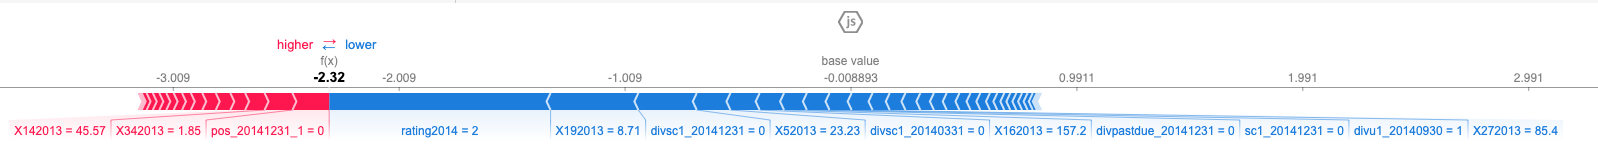
\includegraphics[scale=0.4]{latex/figs/adjusted1_exp.png}
\caption{Explanation of a single negative prediction}
\end{figure}

\begin{figure}[H]

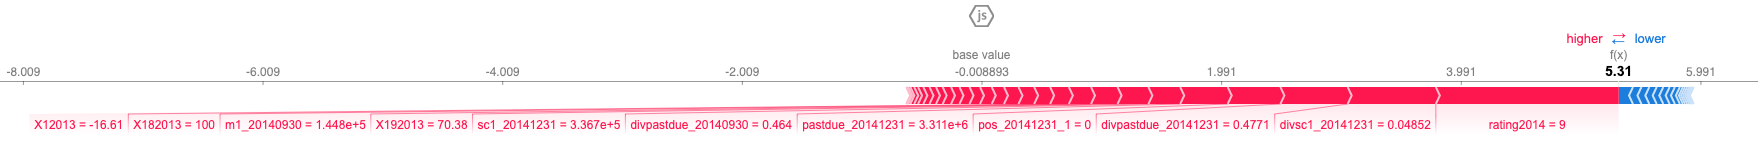
\includegraphics[scale=0.28]{latex/figs/adjusted2_exp.png}
\caption{Explanation of a single positive prediction}


\end{figure}

Finally we consider Adjusted default prediction using only credit data for  the most recent period in which no balance sheet data are available. An analysis of the results obtained using the Catboost classifier are shown in the following figures. Also in this case if we use other classifiers we obtain similar results. We can see that in this case there is a nice balance between the feature of the two datasets. The dominant elements are the probability of default, Unlikely To Pay (inadprob), arrears and the ratio of overdraft over the granted amount (divsc)


\begin{figure}[H]
%\flushleft
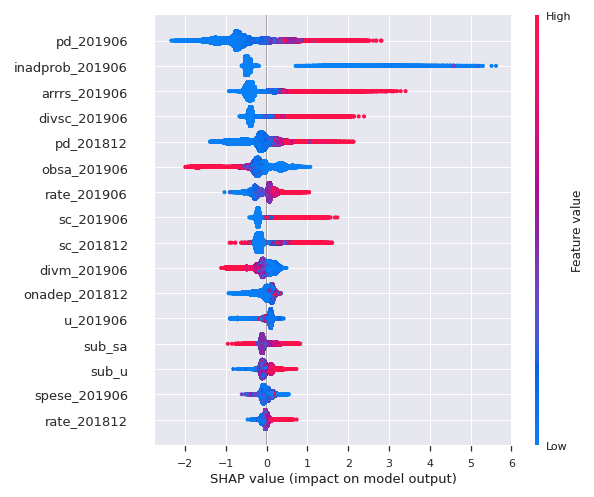
\includegraphics[scale = 0.6]{latex/figs/anac_exp.png}

\caption{Explanatory overview Catboost}
\end{figure}
\begin{figure}[H]
%\flushleft
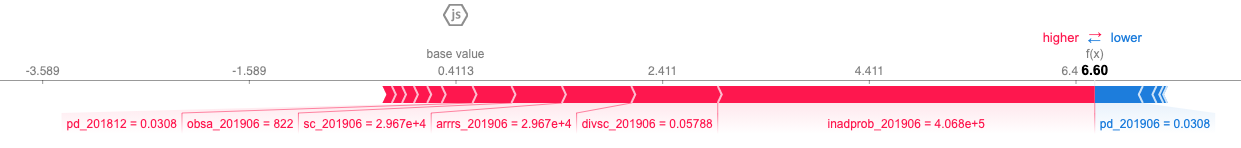
\includegraphics[scale = 0.3]{latex/figs/anac_exp2.png}

In this single prediction explanation is important to notice how despite the fact that the company has the most important attributes, the probability of default, very low it succeed in predicting the company properly basing it on all the other features and showing how they influenced it. 
\caption{Explanation of a single positive prediction}
\end{figure}
\begin{figure}[H]
%\flushleft
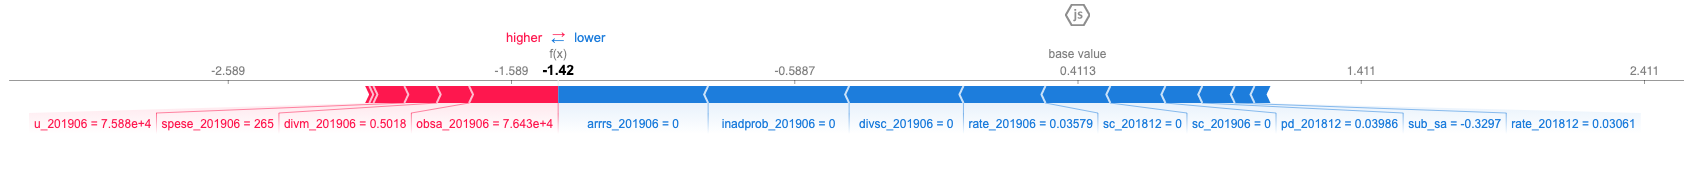
\includegraphics[scale = 0.3]{latex/figs/anac_exp1.png}

\caption{Explanation of a single negative prediction}
\end{figure}

The analysis carried out with SHAP clearly shows some features that are dominant in the forecasts and that belong to both the balance sheet and credit dataset. It seems relevant to us to underline that all these factors can be correlated with potential problems of the company that may be detectable in periods prior to the firms failure.








\section{Conclusion}
\label{sec:conclusion}

Business-failure prediction is a very important topic of study for economic analysis and the regular functioning of the financial system. Moreover the importance of this issue has greatly increased following the recent financial crisis. 
Furthermore, we can certainly consider that the current global crisis caused by Covid-19 will lead to a significant increase in business failures by amplifying the relevance of a good ability to analyze and predict phenomena.

There have been many recent studies that have tried to predict the failure of companies using various machine-learning techniques.
In our study, we used for the first time credit information from the ItalianCentral Credit Register and from ECB AnaCredit survey to predict the banking default of Italian companies, using Machine Learning and other well-known statistical techniques.
We analyzed a very large dataset containing information about almost all the loans of all the Italian companies. Our first findings is that, both in the case of bankruptcy prediction and banks default prediction, machine-learning approaches are able to outperform significantly simpler statistical approaches.


In fact, our results confirm the best performance of Machine learning classifier respect to other well-known statistical methods. In addition we show that some recent types of boosting classifiers obtain the best results. 
 \\
 Furthemore, in this paper we explored the differences and links between corporate failures and bank defaults. We focus our analysis both on bankruptcy, a well-known issue in literature, and on the bank default, which in many cases anticipates the failure of a company. At the same time it represents an important sign of vulnerability as typically a company in bank default is unable to repay its debts.
 \\
 We use Central Credit Register data in combination with balance sheet data in order to predict both bankruptcy and adjusted default. We show that this combination of data can lead to robust performance in prediction. 
 In fact, using information on past loan data is crucial, but the additional use of balance-sheet data can improve classication even further. We show that the combined use of loan data with balanced-sheet data leads to nice performance for predicting default. We also show that using loan data in the prediction of bankruptcy (where, typically, only balance-sheet data are being used) can play an important role.
 The forecast performances obtained are very similar, but a relevant point seems to be that balance sheet data seems to be more suitable for predicting bankruptcies, while the loan data helps to predict bank defaults much better. We corroborate this conjecture also in terms of expainability of the prediction results.
 
 In addition we use, for the first time given the novelty of this source of data, also information data from ECB AnaCredit survey, recently started under the coordination of ECB, in order to improve adjusted default prediction in the more recent years.  We try to exploit the predictive capacity of our credit information by using BORUTA, a  feature selection technique that seems to work very well in our case.
 
 This approach seems to improve prediction performance allowing to obtain remarkable results, with an AuROC of 0.93, even in comparison to the most relevant literature on the subject.
 \\

 Moreover, a relevant point of our work concerns the attempt to explain default predictions; this theme is indeed very relevant for the practical use of forecasting techniques. To this end we used SHAP, a modern method to extract the importance of features in the forecast, showing a robust dependence of our predictions on a series of information that have an important economic significance.
 For example, as easily understood, probability of default (PD) assessed by the banking system play a significant role in a bank default prediction. But a  comparison exercise with the default prediction based only on PD used by banks shows that predictions with Machine learning provide a very significant gain in performance.
 \\
 \\
 Nevertheless, prediction remains an extremely hard problem in this field with very unbalanced dataset. Yet, even slight improvement in the performance, can lead to savings of multiple hundreds of thousands of euros for the banking system. Thus our goal is to improve classification even further by combining our approaches with further techniques, such as neural-network based ones. Some preliminary results in which we use only neural networks are encouraging, even though are worse than the results we report here.
 
 



\begin{comment}

\end{comment}






\bibliographystyle{splncs04}
\bibliography{finance}


\end{document}

